\section{Parser Combitators for Path Querying}

Parser combinators provide a way to specify a language syntax in terms of the functions and operations on them. A parser in this framework is usually a function which consumes a prefix of an input and returns either a parsing result or an error, if the input is erroneous. Parsers can be composed by using a set of parser combinators to form more complex parsers. A parser combinators library provides with a set of basic combinators (such as sequential application or choice), and there can also be user-defined combinators. Most parser combinators libraries, including the Meerkat library, can only process the linear input. We extend the Meerkat library to work on the graph input.

Meerkat library is a general parser combinators library; by using memoization, continuation passing style and ideas of [!!!тут нужна ссылка на johnson!!!] it supports arbitrary context free specifications. This library is closely related to the Generalized LL algorithm and since GLL can be generalized for context free path querying~\cite{GrigorevR16}, the adaptation of Meerkat is reasonable too [!!! Вот тут надо подумать !!!]. 

Let us introduce an example of the same generation query by using Meerkat.
Context-free grammar $G$ presented in Fig.~\ref{fig:query1} and its Meerkat representation is in Fig.~\ref{fig:query1Meerkat}

\begin{figure}[h]
\begin{align*}
& S \rightarrow subClassOf^{-1}\ S\ subClassOf\\
& S \rightarrow type^{-1}\ S\ type\\
& S \rightarrow subClassOf^{-1}\ subClassOf\\
& S \rightarrow type^{-1}\ type
\end{align*}
\caption{Query 1 grammar}
\label{fig:query1}
\end{figure}

\begin{figure}[h]
\begin{lstlisting}
val S: Nonterminal = syn(
   "subclassof-1" ~ S ~ "subclassof" |
   "type-1" ~ S ~ "type" |
   "subclassof-1" ~ "subclassof" |
   "type-1" ~ "type")
\end{lstlisting}
\caption{Meerkat representation of Query 1}
\label{fig:query1Meerkat}
\end{figure}

Let us take a look at it.
For every nonterminal in our CF grammar we create a val of  \lstinline{Nonterminal} type.
Strings are implicitly converted to terminals.
\lstinline{syn} is a macro which creates new nonterminal and automaticaly assigns a name of our val to it.
Inside a \lstinline{syn} macro we have got a defenition of nonterminal.
It uses two combinators \lstinline{~} and \lstinline{|}.
The first one \lstinline{~}  states that after edge described by left operand we would like to have adjacence edge described by right one.
\lstinline{|} is an altenative combinator which have lower priority then \lstinline{~} and used to describes possible alternatives of paths description.

The following table shows some combinators available in Meerkat. 

\begin{table}[h]
\centering
\begin{tabular}{|c|c|}
\hline
\multicolumn{1}{|c|}{Combinator} & \multicolumn{1}{c|}{Description} \\ \hline
{\lstinline!a ~ b!} & {\lstinline!a!} and then {\lstinline!b!}   \\
{\lstinline!a | b!} & {\lstinline!a!} or {\lstinline!b!}         \\
{\lstinline!a.?!}   & {\lstinline!a!} or nothing   \\
{\lstinline!a.*!}   & zero or more of {\lstinline!a!} \\
{\lstinline!a.+!}   & at least one {\lstinline!a!} \\
\hline
\end{tabular}
\caption{Meerkat combinators}
\label{table:combinators}
\end{table}


It can be done by using an odservation which for (string or graph) parsing we need only to provide function for getting symbols follower by specified position.


One of the most excited combinators feature is that queries using combinators can be used as first class values, which provide high ability for queryes generalization and comosition.
Let's take a look at Fig~\ref{fig:gen}. \lstinline{sameGen} creates a same generation query for every pair of brackets in \lstinline{brs}.
This generaization is independent from environment (graph and other parsers), and we can use it for creation of different queries.
For example, the application of \lstinline{sameGen} which one can see in Fig.~\ref{fig:query1Gen} builds a query which is equivalents to the query presented in Fig.~\ref{fig:query1Meerkat}.

\begin{figure}[h]
\begin{lstlisting}
val query1 = syn( sameGen( List(
    ("subclassof-1", "subclassof")
    , ("type-1", "type"))))
\end{lstlisting}
\caption{Application of \lstinline{sameGen} for buildin the query~\ref{fig:query1}}
\label{fig:query1Gen}
\end{figure}

\begin{figure}[h]
\begin{lstlisting}
def sameGen(brs) =
  bs.map { case (lbr, rbr) => 
             lbr ~ syn(sameGen(bs).?) ~ rbr } 
  match {
    case x :: Nil => syn(x)
    case x :: y :: xs => 
      syn(xs.foldLeft(x | y)(_ | _))
  }
\end{lstlisting}
\caption{Generic function for same generations query building}
\label{fig:gen}
\end{figure}

And let us finally parse graph from Fig.~\ref{fig:graph} and get all paths described by same-generation grammar from it.

\begin{figure}[h]

\includegraphics{graph}
\caption{Example graph}
\label{fig:graph}
\end{figure}

To do it let us use meerkat function \lstinline{parseGraphFromAllPositions(parser,graph)} which applies given parser to given graph and gets from SPPF all pairs of nodes such that exists a path between them described by a parser.

The result for graph in Fig.~\ref{fig:graph} is $\{(1,0), (1,2), (0,0), (2,1), (2,2), (0,2), (0,1), (1,1)\}$, where $(i,j)$ stands for the path from node with label $i$ to the node with label $j$

Meerkat library consists of 3 main units (Fig. ~\ref{fig:architecture}): the input data unit, the analysis unit, the visualization unit.

The input data unit can accept two main types: graphs and strings. It is necessary to implement the IGraph interface to analyze graphs with different implementations. There are two implementation of IGraph at the moment: Neo4JGraph and SimpleGraph. Neo4JGraph takes data from the Neo4j graph database. SimpleGraph allows you to describe the graph in the code of the program.

The analysis unit consists of parser and SPPFLookup. The parser gets the input data and the grammar, which is a input data query.  The parser maps the input data to the input grammar and finds all the paths. The result is added to the SPPFLookup data structure, which contains all the paths in the input data corresponding to the grammar. All nodes in the SPPFLookup are in a single instance and re-used.

After the analysis is completed, the visualization unit gets SPPFLookup and SPPF query. The unit filters the path and then returns the file in dot format to the user.
%\begin{figure}
%\caption{Architecture Meerkat}
%\label{fig:architecture}
%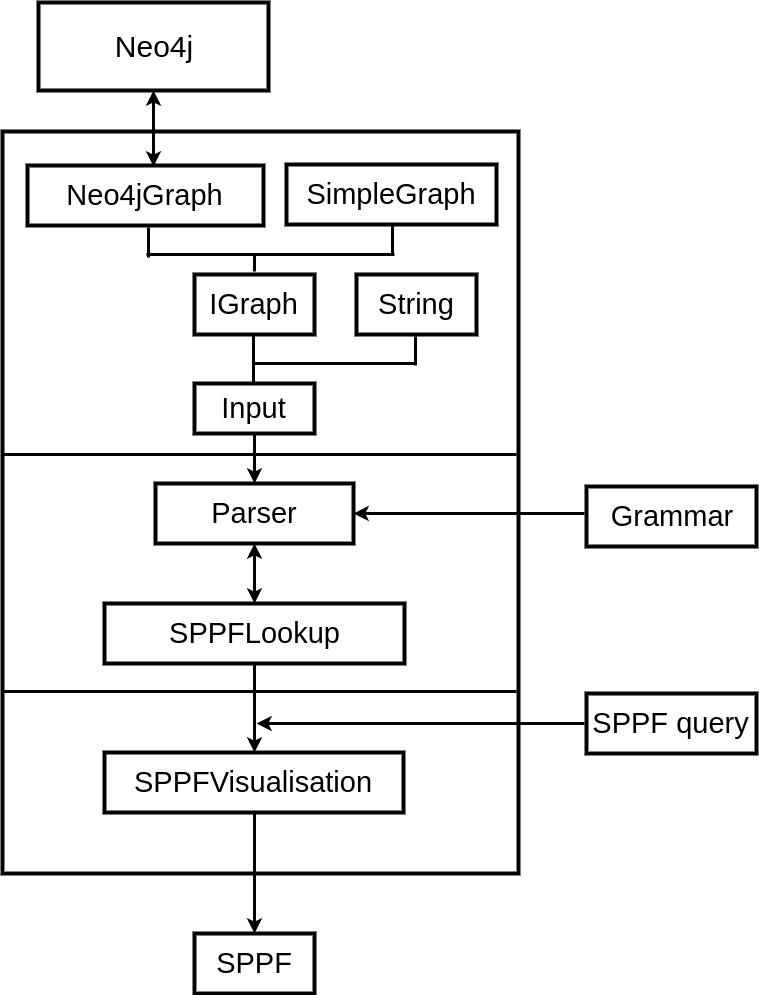
\includegraphics[width=0.3\textwidth]{architecture.jpg}
%\end{figure} 




